% Source page: original p. 343 (PDF p. 39)
% Figure number: Figure 15
% Uncertainty notes: The scan is slightly soft; the dotted classical potential is rendered as nearly horizontal, and the solid effective potential is reconstructed as the peaked profile visible in the source.
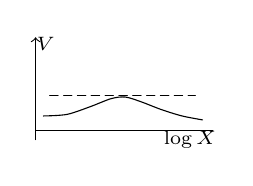
\begin{tikzpicture}[x=1cm,y=1cm,line cap=round,line join=round]
  \draw[->] (0,-0.02) -- (0,1.28);
  \draw (0,0.10) -- (2.25,0.10);

  \node[font=\scriptsize] at (0.13,1.20) {$V$};
  \node[font=\scriptsize] at (1.96,-0.02) {$\log X$};

  \draw[densely dashed] (0.18,0.54) -- (2.03,0.54);

  \draw[smooth] plot coordinates {
    (0.10,0.28) (0.40,0.30) (0.70,0.40) (0.96,0.50)
    (1.14,0.52) (1.34,0.46) (1.60,0.36) (1.86,0.28) (2.12,0.23)
  };
\end{tikzpicture}
